\documentclass[12pt,a4paper]{amsart}

\usepackage[english]{babel}

\usepackage{amssymb,amsmath,amsfonts,amsthm}
\usepackage{graphicx}
\graphicspath{{./figures/}}
\usepackage[left=1in,right=1in,top=1in,bottom=1in]{geometry}

% Bibliography Style:
\usepackage[sort&compress,round]{natbib}
\setlength{\bibsep}{1ex}
\setlength{\bibhang}{1cm}

%\renewcommand{\baselinestretch}{2.0}

\usepackage{hyperref,url}
%\usepackage{pstricks,pst-node,pst-tree}

%\input xy
%\usepackage[cmtip]{xypic}
%\xyoption{all}
%\CompileMatrices

%\usepackage{newicktree}


\usepackage{array}
\usepackage{bm}
\let\empset\emptyset


\newtheorem{thm}{Theorem}
\newtheorem{lemma}[thm]{Lemma}
\newtheorem{prop}[thm]{Proposition}
\newtheorem{cor}[thm]{Corollary}
\newtheorem{prob}[thm]{Problem}
\newtheorem{conj}[thm]{Conjecture}
\newtheorem{alg}[thm]{Algorithm}
\newtheorem{rmk}[thm]{Remark}

\newtheorem{ex}[thm]{Example}
\newtheorem{df}[thm]{Definition}

\newcommand{\eps}{\varepsilon}
\newcommand{\cE}{\mathcal{E}}
\newcommand{\cG}{\mathcal{G}}
\newcommand{\NN}{\mathbb{N}}
\newcommand{\RR}{\mathbb{R}}

\newcommand{\cA}{\mathcal{A}}
\newcommand{\cC}{\mathcal{C}}
\newcommand{\cS}{\mathcal{S}}
\newcommand{\cX}{\mathcal{X}}
\newcommand{\cY}{\mathcal{Y}}
\newcommand{\cZ}{\mathcal{Z}}
\newcommand{\Data}{\mathcal{D}}
\newcommand{\indep}{\perp}

\DeclareMathOperator{\pa}{pa}
\DeclareMathOperator{\E}{E}
\DeclareMathOperator{\Var}{Var}
\DeclareMathOperator{\Cov}{Cov}

\DeclareMathOperator{\HW}{HW}
\DeclareMathOperator{\Norm}{Norm}
\DeclareMathOperator{\Bern}{Bern}
\DeclareMathOperator{\Binom}{Binom}
\DeclareMathOperator{\Bernoulli}{Bernoulli}
\DeclareMathOperator{\Mult}{Mult}
\DeclareMathOperator{\Dir}{Dir}
\DeclareMathOperator{\Exp}{Exp}
\DeclareMathOperator{\Exit}{Exit}
\DeclareMathOperator{\Pois}{Pois}
\DeclareMathOperator{\MC}{MC}
\DeclareMathOperator{\Model}{M}
\DeclareMathOperator{\pos}{pos}
\DeclareMathOperator{\nt}{nt}


% For editing:
\usepackage{lineno}
\usepackage{color}
\newcommand{\niko}{\textcolor{red}}
\usepackage[colorinlistoftodos]{todonotes} 

\begin{document}

%\linenumbers
%\modulolinenumbers[2]

\title{A probabilistic model for reconstructing intra-tumor phylogenies}



\author{
NB-lab + FM-lab
}

\date{\today}

\begin{abstract}
We present an intra-tumor oncogenetic tree (ITOT) model for inferring tumor evolutionary histories from NGS data obtained from bulk sequencing of mixed tumor samples.
%We extend phylogenetic methods to infer cancer evolutionary trees from deep-sequencing data. 
Our methods not only infer the number of clones per sample but also the most likely life history of the tumor.
Our methods allow us to (i)~infer early events in tumour development, (ii)~link cancer heterogeneity to clinical outcome, (iii)~compare clonal evolution in metastasis to evolution in the primary tumour.
\end{abstract}


\maketitle


%%
%%
%%%%%%%%%%%%%%%%%%%%
%% INTRODUCTION
%%%%%%%%%%%%%%%%%%%%
%%
%%

\section{Introduction}

Cancers are heterogenous, the usual bla bla \cite{Shah2009,Nik-Zainal2012,Nik-Zainal2012a,Aparicio2013}

Progress has been made on clustering sequencing data into clonal subpopulations (\cite{Shah2012}, Ben Raphael's TheTA, Perou+Mardis paper soon), but the evolutionary relationships between these clones, the so called life history of a cancer, has so far only been estimated by eye \citep{Nik-Zainal2012a}. 

To change this sad situation, we need rigorous and accurate phylogenetic methods to automate the inference of the evolutionary history of a tumor. 
These methods will enable us to infer early driver events on a large scale, test whether evolutionary trajectories are predictive of outcome, and compare clonal evolution between pimary and metastatic tumors.
%The link between patient-specific clonal evolution and clinical outcomes like relapse or progression-free survival has not been rigorously tested. 
Better phylogenies will improve the usefulness of all cancer heterogeneity studies, which so far are limited to enumerating longer and longer lists of mutations and aberrations.
Our work extends methods proposed in \cite{Schwarz2013a,Schwarz2013b} from multiple-sampled copy-number profiles to SNVs from deep-sequencing data.

%We would like to reconstruct the evolutionary history of individual tumors. 
%Each tumor consists of multiple subclonal genetic variants that have evolved after its last clonal expansion. 
We assume that the mixed tumor cell population has been bulk sequenced, such that the resulting reads provide a statistical sample of the underlying population.
Ignoring structural variation and copy number alterations, we aim at inferring a phylogenetic tree model that represents the evolutionary history of the tumor clones from the observed short read data focusing only on single-nucleotide variations (SNVs). 
This task is different from classical phylogenetic approaches in at least three ways: 
(i) The observed data are short reads covering only a small fraction of the cancer genotypes that define the subclones. 
(ii) Due to the bulk sequencing approach of mixed samples, it is unknown which read originated from which cancer genotype. 
(iii) Read counts allow for inference of relative frequencies of mutations, which are informative about the order in which mutations have occurred.   

The starting point of our method development will be existing methods for estimating clonal populations. 
A prominent example is pyclone \citep{Shah2012}, which corrects mutation frequencies for copy number alterations and loss of heterozygosity and clusters the frequency distribution using a Dirichlet process mixture model. 
The outcome of this analysis is the number of clones and their frequencies; what is still unknown is the evolutionary history of the clones and previous approaches have relied on visual analysis to place clones in a phylogenetic tree \citep{Nik-Zainal2012a}. 

We will automate this process by implementing the key ideas of \citet{Nik-Zainal2012a}  in a rigorous statistical model. 
The central insight is that the way clonal frequencies add up hints at their evolutionary history. 
Figure~\ref{fig1}A illustrates this idea in an idealized scenario by showing how a population of three clones (with genotypes A, BC, BD) results in a mutation frequency distribution with four peaks (centred around the frequencies of A,B,C,D). 
The tree structure is reflected in the frequency distribution: frequencies of A and B add up to 100\% and frequencies of C and D add up to the frequency of B, their ancestor in the tree. \todo{this might be a bit too constrained} 
However, in noisy data these relationships can be blurred, which makes tree construction difficult. 
In particular, the clustering could result in spurious clusters or misplaced cluster centers that cannot be fit in a tree. 
This is the reason why in the manual reconstruction in \cite{Nik-Zainal2012a} one of the big clusters had to be split by hand into three smaller ones that were attached to different parts of the tree.

\begin{figure}[t]
\centerline{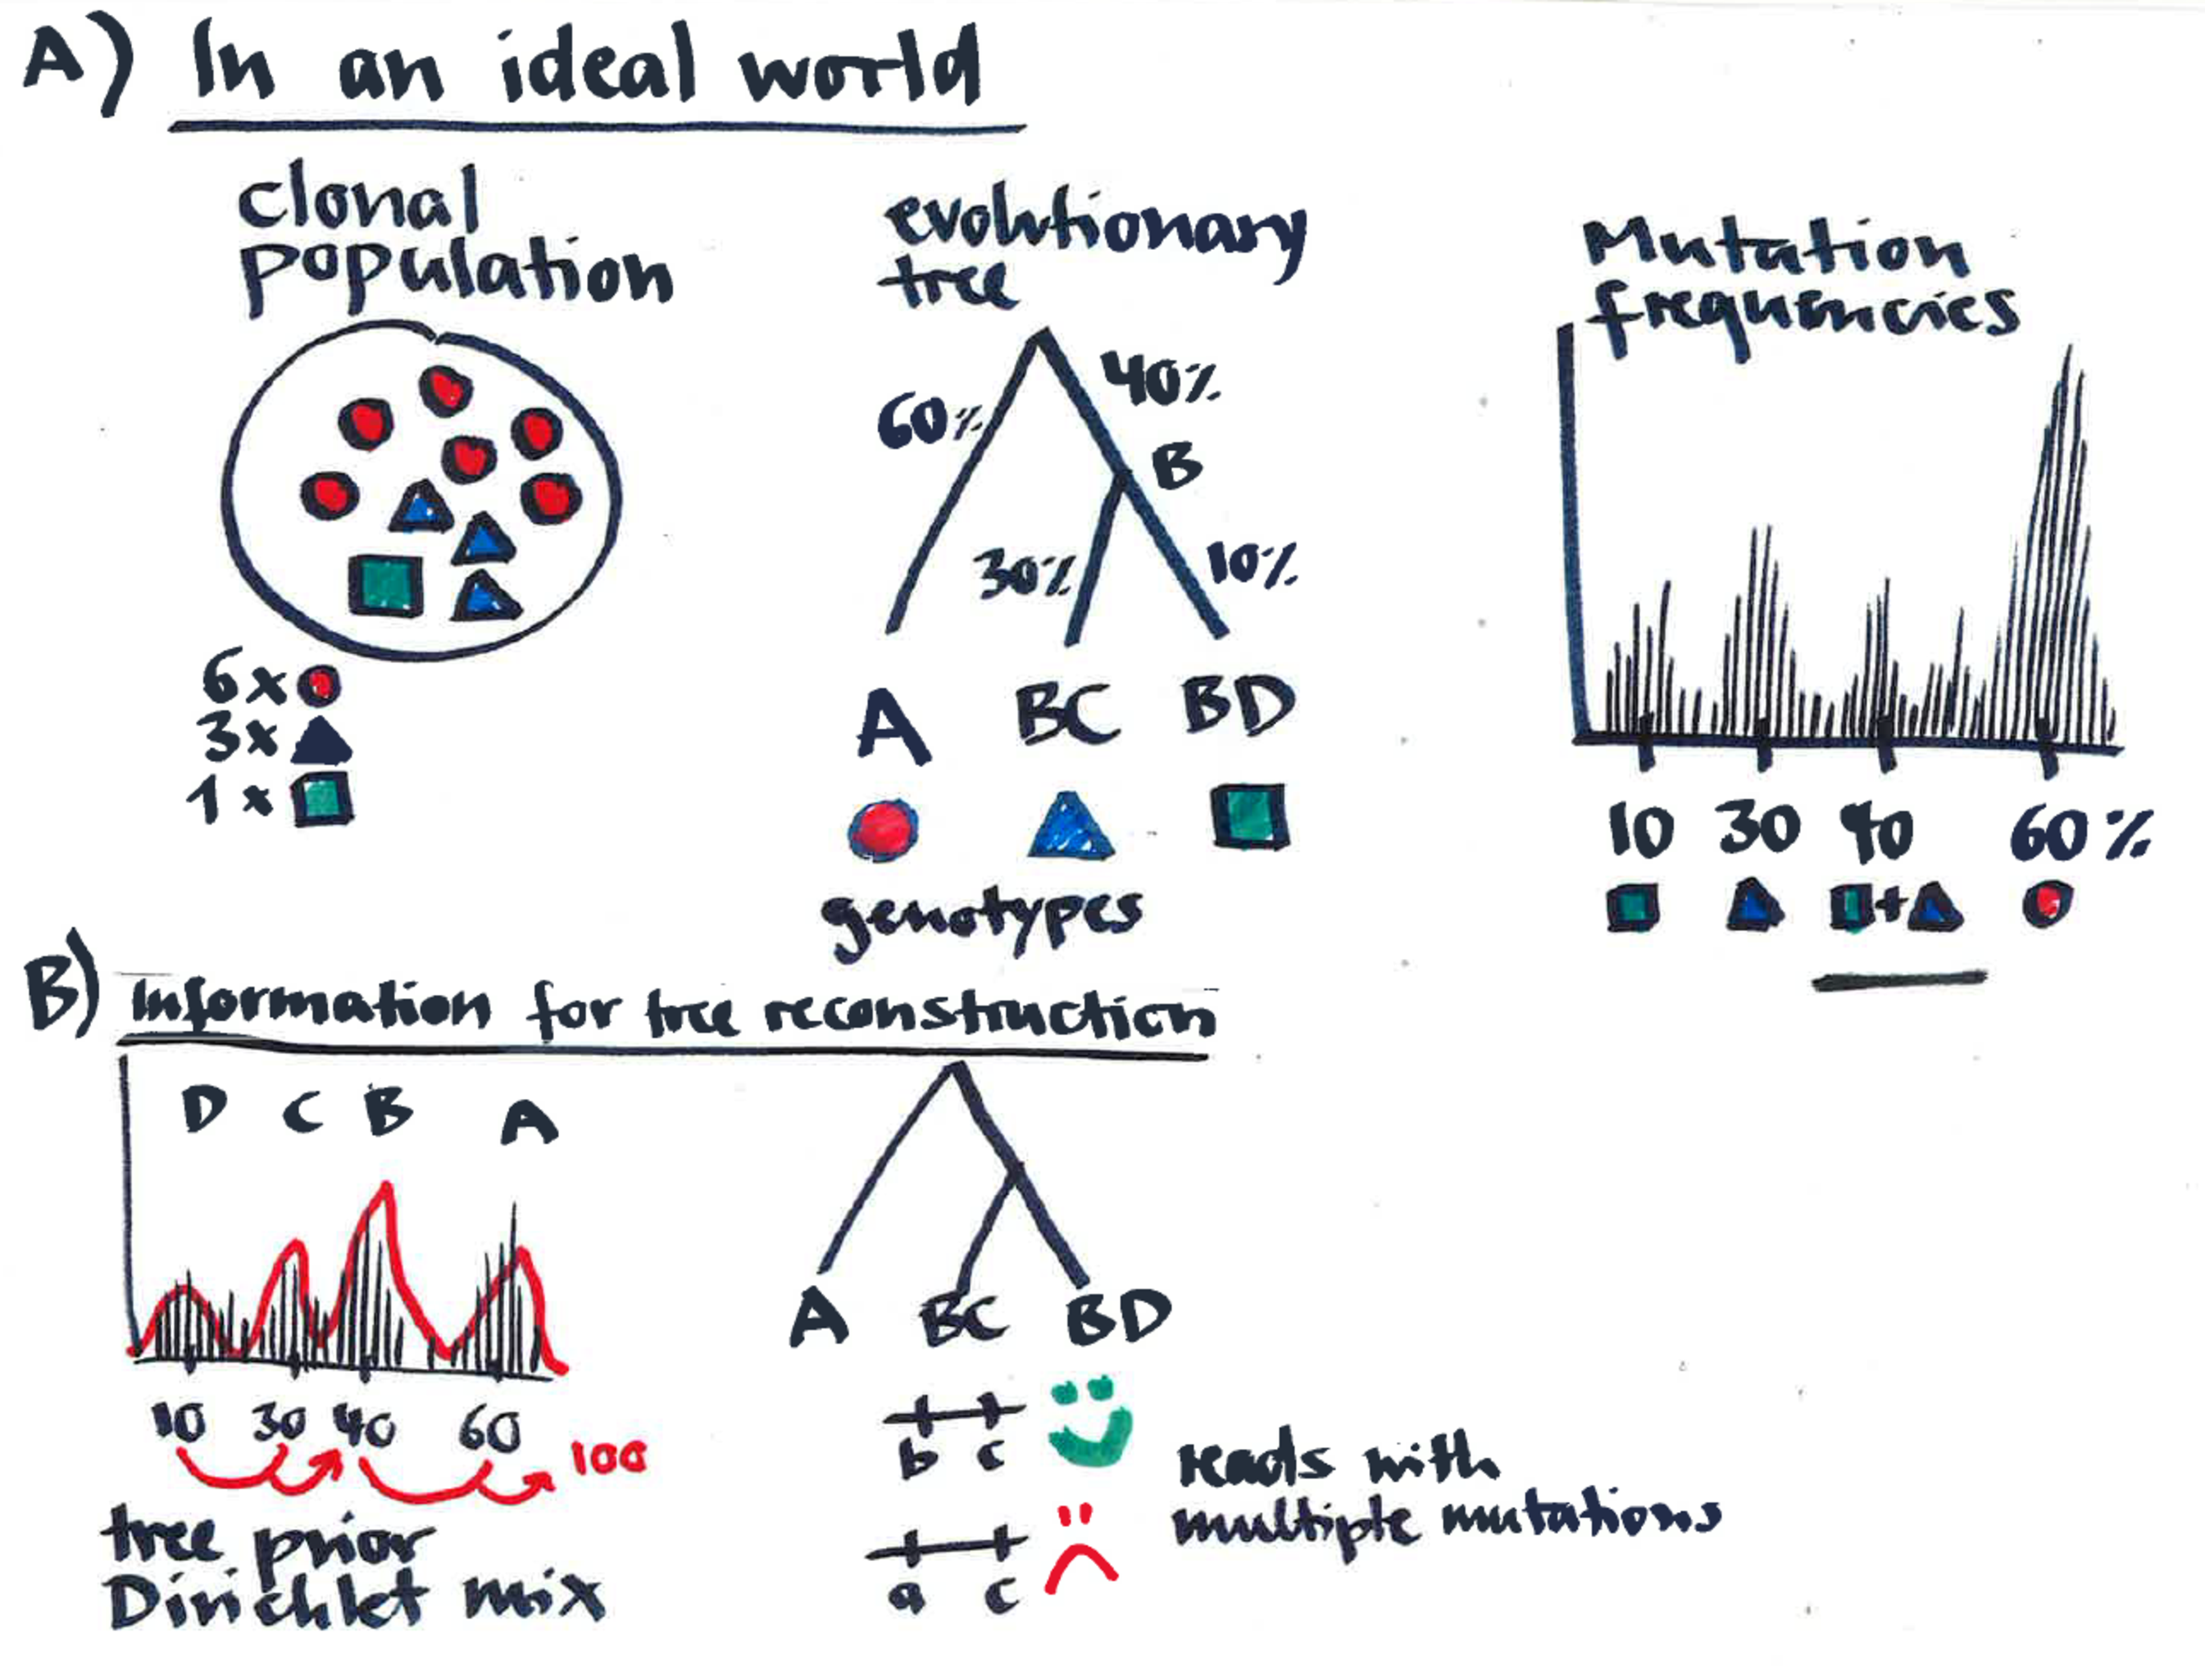
\includegraphics[width=.9\textwidth]{fig1}}
\caption{\textbf{A)} Overview how heterogeneity in a tumor relates to clonal evolution and is reflected in mutation frequencies. \textbf{B)} The sources of information we have available for inference.}
\label{fig1}
\end{figure}

To address these problems, we propose the following approach. 
We will start by calling mutations from deep-sequencing data and correcting their frequencies for copy-number and loss of heterozygosity in the same way as pyClone. 
To infer clonal evolutionary trees we will use two complementary pieces of information (Figure~\ref{fig1}B): First, we will constrain the clustering of mutation frequencies to ensure that clonal frequencies are �tree-like�. 
Instead of sequentially clustering and tree-building we will combine both steps into a single model, following ideas of \citet{Adams2010,Williams1999}.
As a result our mixture model will automatically (1) estimate the number of clones and (2) place them in an evolutionary tree. 

A second source of information to validate this tree are the reads that contain more than one mutation. 
In the example of Figure~\ref{fig2} reads with mutations from both B and C would agree with the tree, but all reads with mutations from A and C would be evidence against it. 
Our final model will integrate the tree-constrained clustering with the information in multiply mutated reads into a joint likelihood to estimate the most likely tree topology.

\section{Our goals}

\begin{figure}[b]
\centerline{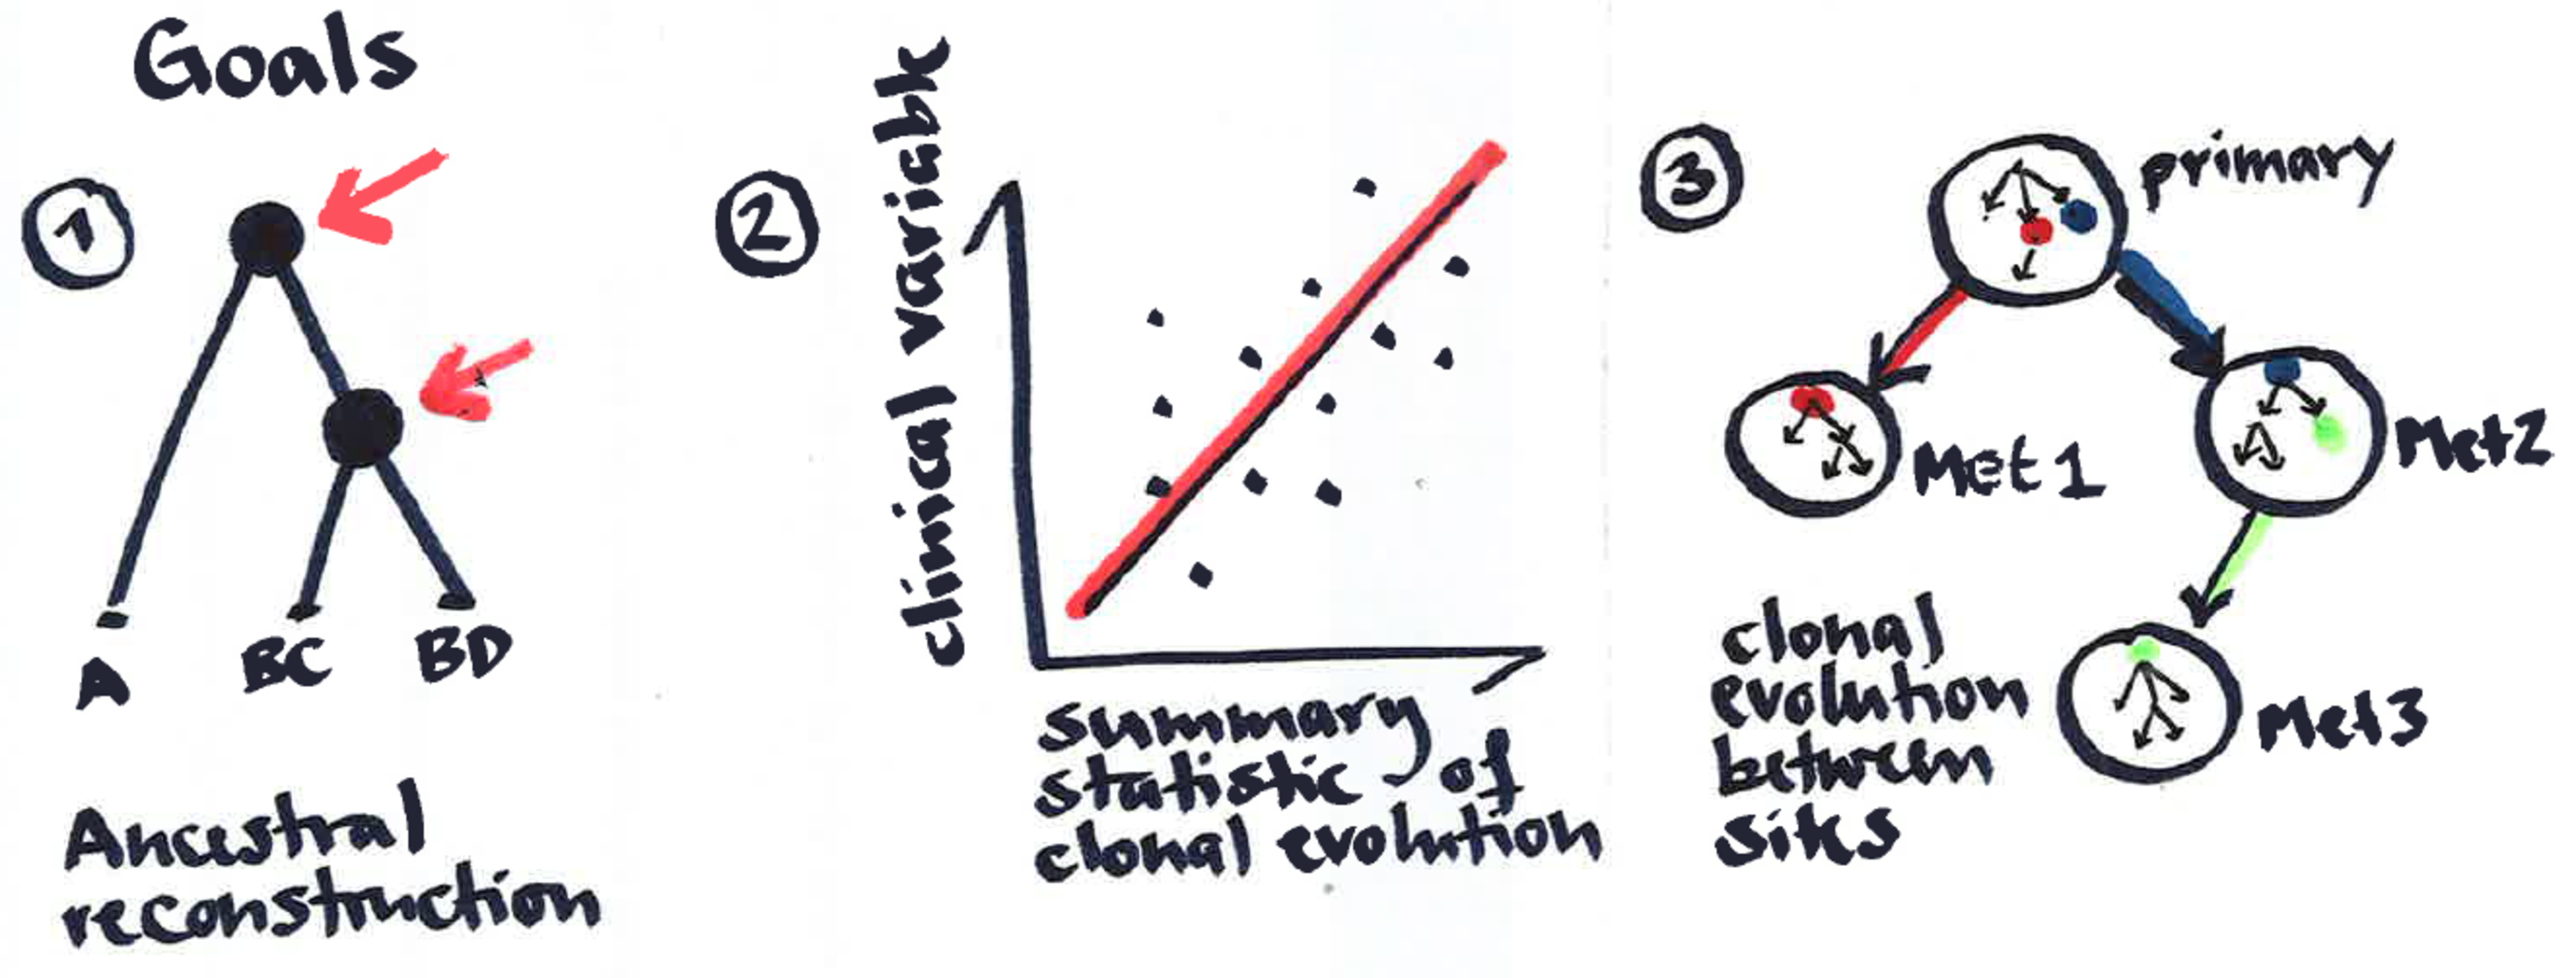
\includegraphics[width=.9\textwidth]{fig2}}
\caption{\textbf{Goals of our analysis are} (i)  to infer early events in tumour development, (ii) to link cancer heterogeneity to clinical outcome, (iii) to compare clonal evolution in metastasis to evolution in the primary tumour.}
\label{fig2}
\end{figure}


Our method will allow us to investigate three pivotal questions:

\subsection*{1. In which order did genomic events occur during tumor development?}
Earlier driver events will be more important drug targets than newer ones.
To time events, our first goal will be to automate the phylogenetic inference of clonal evolution, as exemplified in Nik-Zainal et al (2012).

We will validate our approach using simulations of tumour evolution driven by basic biological principles, following the ideas developed in \cite{Schwarz2013a}. 

This project will be our main focus in the beginning. Once the model is established, the next project is basically for free (except for the blood, sweat and tears of applying it).

\textbf{Data:} We will use the data of \citet{Nik-Zainal2012} to compare our automatically reconstructed trees to their visual analysis. \todo{Are there any other clonal trees out there that we could compare against?}

\subsection*{2. How predictive are �life histories� of tumours for clinical endpoints?}
In esophageal adenocarcinoma measures of clonal heterogeneity (entropy: number of clones weighted by their frequency) predict disease progression \citep{Maley2006}.
This is a landmark study, because the link between heterogeneity and clinical variables is still widely unexplored.
\citet{Maley2006} identified clones by any difference in flow cytometric DNA content (for differences 40.2N), LOH, microsatellite shifts (new alleles) and CDKN2A or TP53 sequence mutations.

We will extend the analysis of \citet{Maley2006} to deep sequencing data.
Using the trees from our method we will compute summary statistics that measure genomic heterogeneity of the tumor and quantify features of its evolutionary history. The simplest summary statistics (and baseline of our analysis) are the number of clones and entropy of their distribution \citep{Maley2006}, which do not take any features of the tree into account. Our hypothesis is that measures of heterogeneity, which explicitly rely on features of the tree structure, are more informative than the number of clones.

\textbf{Data:} We will apply our method to the 65 triple-negative breast cancers sequenced in \cite{Shah2012}, for which clinical data is available. \todo{We can already now conpute clonal distribution + entropy for all theses samples (as Shah et al have done already) and correlate with outcome.} We will also need a validation set of at least equal size.\todo{Where do we get this?} We can use all available data from all cancers. Being able to compare the predictive power of trees between cancer types would make us stronger. \todo{Collect all data!}
 
\subsection*{3. How does clonal evolution in the patient span primary tumour and metastases?}
In a (so far) unpublished project Elaine Mardis and Chuck Perou work on data of sequencing samples of a primary breast tumour and five metastases at different anatomical sites. They clustered sequencing data into clones individually for each sample and ordered the samples into a tree using Phylip on the average genomic profile. 

We will algorithmically improve this analysis by developing methods for joint inference of sample-specific trees and a global tree, which together will show how clones evolve within a tumor and spread to other anatomical sites to start a metastasis. This approach will �borrow information� across samples to identify small clonal subpopulations that might be missed if samples are treated independently.

The goal is to infer clonal evolution in the patient, spanning different anatomic sites and showing how clones move from one site to the next and populate a metastases.

\textbf{Data:} These data are not yet published, but Mardis is giving talks -- can't be long. It would be good to have a basic method ready when the data come out.

\section{How to get started}

\begin{itemize}
\item First step: during Thomas' visit we will start merging our methodological ideas (see below) and derive a battle plan for method development. DONE!
\item Repository for  code, manuscripts and data(?). Any objections to using bitbucket? DONE!
\item Data collection: these genetic data take a while to collect because of all the bureaucratic hoops to jump through. We need to start now basically even if we don't plan to touch them for months.
\item Regular meetings. Every two weeks? MOSTLY EMAIL. SKYPE MEETINGS WHEN MILESTONES ARE REACHED. NEXT MILESTONE: RECONSRUCT NIK-ZAINAL TREE.
\end{itemize}


%%
%%
%%%%%%%%%%%%%%%%%%%%
%% METHODS
%%%%%%%%%%%%%%%%%%%%
%%
%%



\section{Methods}
We assume the sequencing data is restricted to loci with clonal
monosomies. Furthermore, each read is overlapping with two SNV positions, but
does not necessarily contain the two or one 
SNV.  
Considering the Bayesian nonparametric approach introduced in \cite{Adams2010}
we construct two (alternative) models: 

\subsection{Pairing models}

\paragraph{\it{Factored Bernoulli likelihood-based approach} }
The data consists of two-dimensional binary vectors indicating the statuses of
the SNVs covering this read and two genomic positions indicating the positions
of those two SNVs: 
$X_n \in (\{0,1\}^2,position1, position2)$

The node wise likelihood is parametrized by a latent two-dimensional real vector
which is then component-wise logit transformed:  
$\theta_{\epsilon} \in \RR^N$

$N$ is the length of the genomic loci of interest or the cardinality of $\cS$.

\begin{align}
f(x_n\mid\theta_{\epsilon})=(1+exp(-\theta_{\epsilon})^{(position1)})^{-x_n^{(1)}})*(1+exp(\theta_{\epsilon})^{(position1)})^{1-x_n^{(1)}})*\\ 
(1+exp(-\theta_{\epsilon})^{(position2)})^{-x_n^{(2)}})*(1+exp(\theta_{\epsilon})^{(position2)})^{1-x_n^{(2)}})*\\ 
\frac{1}{N*(N-1)} 
\end{align}

The transition kernel consists of a product of independent Gamma distributions: 

\begin{equation}
T(\theta_{ \epsilon \epsilon_i}\leftarrow \theta_{\epsilon})=\prod_{j=1}^{N} Gamma(\theta_{ \epsilon \epsilon_i}^{(j)} - \theta_{\epsilon}^{(j)} \mid \alpha,\beta)
\end{equation} 

The root level prior:

$p(\theta_0)=$distribution that fits the clonal SNVs of interest

\paragraph{\it{Discrete SNV-pool-based approach}}
$\cS$ contains all identified clonal and subclonal SNVs in the loci of interest. 

$\eps$ is the global error parameter.

The data is structure similar to the Factored Bernoulli likelihood-based approach:
$X_n \in (\{0,1\}^2,position1, position2)$

The node wise likelihood is parametrized by a latent SNV set containing a subset of $\cS$:
$\theta_{\epsilon} \in \cS$

The node wise data likelihood is define as:
\begin{eqnarray}
	f(x_n \mid \theta_{\epsilon}) &=&
		\begin{cases}
			\eps^2        & \text{if $|\{s,t\} \cap \theta_{\epsilon}| = 0$} \\
     		2\eps(1-\eps) & \text{if $|\{s,t\} \cap \theta_{\epsilon}| = 1$} \\
     		(1-\eps)^2    & \text{if $|\{s,t\} \cap \theta_{\epsilon}| = 2$}
		\end{cases}
\end{eqnarray}

The transition kernel adds a random subset of $\cS$ without the parent SNVs $\theta_{\epsilon}$ and adds them to the child SNV set $\theta_{ \epsilon \epsilon_i}$:

\begin{equation}
T(\theta_{ \epsilon \epsilon_i}\leftarrow \theta_{\epsilon})=MUT(\theta_{ \epsilon \epsilon_i} \mid \theta_{ \epsilon }, \cS)
\end{equation}
 
$MUT$: a random number of elements of the set $\cS \\ \theta_{ \epsilon }$ is chosen. PMF: combinatorial

The root level prior:
$p(\theta_0)=$distribution that fits the clonal SNVs of interest

\subsection{The frequency models}

The frequency data could use either Binomial ( including PyClone) or Gaussian variables.

For the Binomial model, the data takes the following format, $X_n \in \{{y_n, q_n}
\in \mathbb{N}, s \in \cS\}$. The likelihood is:
\begin{align}
   f(x_n |\theta_{\epsilon})= \mbox{Binomial}(y_n | q_n, \theta_{\epsilon})  
\end{align}

The cellularity can be used to scale $\theta_{\epsilon}$. For PyClone, the
parameter $\theta_{\epsilon}$ becomes a function of copy number state and others.

For the Gaussian model, the data becomes  $X_n \in \{x_n \in
[0,1], s \in \cS\}$. The likelihood is:
 \begin{align}
    f(x_n |\theta_{\epsilon} ) = \mbox{Normal}( x_n | \theta_{\epsilon}^{(1)}, \theta_{\epsilon}^{(2)}  )
  \end{align}

Similarly, the cellularity can also be use to scale $\theta_{\epsilon}$.

\paragraph{\it{Priors}}
The frequency models share the same transition kernel is the same as Eq. 
\begin{equation}
T(\theta_{ \epsilon \epsilon_i}\leftarrow \theta_{\epsilon}) =
\mbox{Beta}\left(\frac{\theta_{ \epsilon \epsilon_i}}{\theta_{ \epsilon}}
\Big| \alpha, \beta \right) 
\end{equation} 

The root level prior
\begin{align} 
P(\theta_0) = \mbox{Normal} (\theta_0 | \mu, \sigma^2 )
\end{align}
where, $\mu$ is close to $1$, $\sigma^2$ is small.



\subsection{Construct a prior from the frequency model for the pairing model}
Form the results from a frequency model, based on the MAP solution, we have a
label $c_n$ for each SNV. Let 
the depth of the node in pairing model tree be $d = |\epsilon|$, we can get all
the SNVs which are at corresponding location in the frequency model tree. 
$ n \in \{ |c_n| = \{d, d \pm 1\} \}$
 

For the transition kernel, 
\begin{align}
  T(\theta_{\epsilon \epsilon_i} \leftarrow \theta_{\epsilon})
= \prod_{j=1}^{N} \mbox{Gamma}(\theta_{\epsilon \epsilon_i}^{(j)} -
\theta_{\epsilon}^{(j)} 
\mid \alpha_j,\beta_j)
\end{align}
where 
\begin{align}
  \alpha_j, \beta_j = \begin{cases}
  1.5, 0.05 & \mbox{if } j \in \{ |c_j| = d-1 \} \\
  1.5, 0.1 & \mbox{if } j \in \{ |c_j| = d\} \\
  1.5, 0,05 & \mbox{if } j \in \{ |c_j| = d+1 \} \\
  1,   0.05 & \mbox{otherwise} 
\end{cases} 
\end{align}

$p(\theta_0)=$distribution that fits the clonal SNVs of interest




\section{Results}


\section{Discussion}





%%
%%
%%%%%%%%%%%%%%%%%%%%
%% RESULTS
%%%%%%%%%%%%%%%%%%%%
%%
%%

%\section{Results}


%\section{Discussion}




%%
%%
%%%%%%%%%%%%%%%%%%%%
%% REFERENCES
%%%%%%%%%%%%%%%%%%%%
%%
%%
\bibliographystyle{abbrvnat}
\bibliography{./references/ITOT}

%%
%%
%%%%%%%%%%%%%%%%%%%%
%% The end, my friend!
%%%%%%%%%%%%%%%%%%%%
%%
%%
\end{document}
